\documentclass[11pt]{article}
\usepackage{geometry}                % See geometry.pdf to learn the layout options. There are lots.
\geometry{letterpaper}                   % ... or a4paper or a5paper or ... 
%\geometry{landscape}                % Activate for for rotated page geometry
%\usepackage[parfill]{parskip}    % Activate to begin paragraphs with an empty line rather than an indent
\usepackage[pdftex]{graphicx}
\usepackage{amssymb}
\usepackage{epstopdf}

\usepackage[T1]{fontenc}
\usepackage[scaled=0.8]{beramono}

%\DeclareGraphicsRule{.tif}{png}{.png}{`convert #1 `dirname #1`/`basename #1 .tif`.png}
\usepackage{listings} 

\lstset{%
  frame=none,
  xleftmargin=5pt,
  stepnumber=1,
  numbers=left,
  numbersep=5pt,
  numberstyle=\ttfamily\tiny,
  belowcaptionskip=\bigskipamount,
  captionpos=b,
  escapeinside={<|}{|>},
  tabsize=2,
  emphstyle={\bf},
  commentstyle=\it,
  stringstyle=\mdseries\ttfamily,
  showspaces=false,
  keywordstyle=\bfseries,
  morekeywords={in,do,print},
  columns=flexible,
  basicstyle=\sffamily,
  showstringspaces=false,
  morecomment=[l]\%,
}

\lstdefinelanguage{Enso}{%
  numbers=none,
  sensitive=true,
  morecomment=[l]{//},
  morecomment=[s]{/*}{*/},
  morestring=[b]",
  emphstyle={\bf},
  commentstyle=\it,
  stringstyle=\mdseries\ttfamily,
  showspaces=false,
  basicstyle=\ttfamily,
  morekeywords={schema,type},
  keywordstyle=\bfseries,
  columns=flexible,
  showstringspaces=false,
  morecomment=[l]\%,
}

\newcommand{\C}{\lstinline}

\lstset{language=Enso}

\newcommand{\Enso}{Ens\={o}}

\title{
\includegraphics[scale=0.25]{enso.jpg}\\\Enso}
\author{William R. Cook and Tijs van der Storm}
%\date{}                                           % Activate to display a given date or no date

\begin{document}
\maketitle
%\section{}
%\subsection{}


\Enso\ is a theoretically sound and practical reformulation of the 
concepts of model-driven software development. \Enso\ is based
on first-class \textit{structural descriptions}, 
invertable \textit{transformations}, \textit{generic operations} 
and \textit{interpretation}.

Structures in \Enso\ are a specialized kind of graph,
whose nodes are either primitive data or collections of observable
properties, whose values are either nodes or collections of nodes.
From a programming language viewpoint this may seem an odd 
choice for data representation. However, it is essentially the
Entity-Relationship (ER) model \cite{FOO}, also known as Information
Models \cite{FOO}, which is widely used in the design of relational databases
and is also the basis for Class Diagrams in 
the Unified Modeling Language (UML) \cite{FOO}, which 
describe the structure of networks of objects.
The key point is that structures in \Enso\ are 
viewed holistically as \textit{graphs}, not as individual values
or traditional sums-and-products data structures.

A structural description, or \textit{schema}, specifies some 
of the observable properties of structures. Schemas are used to
check the consistency structures. Some properties can be checked
while the structure is being created, but other can only be checked
once the structure is complete. \Enso\ allows modification of structures,
which is necessary to create cyclic graphs, but also allows 
valid structures to be sealed to prevent further changes.

Invertible transformations are used to map one structure into
another kind of structure, such that mapping can be inverted to 
(partially) recover the original structure from the result.
One common kind of transformation is called a \textit{grammar},
which is an invertible transformation between structures and text.
Text grammars are invertable because they can be used for parsing
and also rendering. Other transformations include Diagram grammars,
which map structures into diagrams, were edits on the diagram are
reflected in the original structure. Grammars that describe
the structure and behavior of user interfaces are used to generate
very natural applications.
Transformations are also used for querying, template processing, 
and serialization.

Operations can be guided by schemas or grammars, allowing highly
generic operations to be defined for comparison, differencing, 
merging, projecting and otherwise manipulating cyclic structures.
These operations are cyclic maps, which correspond to coinductive 
transformations.
Since schemas and transformations are also structures, they can
be merged and transformed using these same generic operations.
Transformations on schemas can be applied to instances, to support
upgrade and change management of data.
The resulting system supports powerful modularity constructs,
including feature modules, inheritance, and mixins.

\Enso\ is based on interpretation rather than code generation. 
While it is possible to define transformations that generate code
in conventional languages, this is rarely (if ever) done in \Enso.
Instead all structural descriptions and transformations are 
interpreted dynamically. Although the current incarnation of \Enso\
does not include it, we have previously demonstrated that partial
evaluation can be applied to \Enso-style interpreters to automatically
generate efficient code.

What follows is a rapid introduction to the concepts and use of
\Enso. To avoid too many digressions, 
the many connections between \Enso\ and existing approaches,
including programming models
(model-driven, object-oriented, polytypic, functional, constraint-based), theory (dependent types, coalgebra, category theory),
and related ideas (relational databases, domain-specific languages)
are discussed in Section~\ref{relatedwork}.

\section{Structures}

\subsection{Schemas}

The following schema describes a collection of genealogy information:

\begin{verbatim}
schema GenealogySchema

  class Genealogy
    name: str
    members: Person*

  class Person
    name: str (key)
    birth: date
    female: bool
    father: Person?
    mother: Person?
\end{verbatim}

In a schema, a \textit{class} defines a kind of value, which is
followed by its properties or \textit{fields}. Each field has a name
and a type, where the type may be followed by \C|*| to indicate a 
many-valued field, or by \C|?| to indicate an optional value.
In this case, \C|Genealogy| has \C|members| which is a set of \C|Person|.
A \C|Person| has a \C|name| string, a \C|birth| date, and a \C|father| and \C|mother|,
which are optional \C|Person|s. The \C|father| and \C|mother| are optional
because every geneology is partial, so that not all fathers and mothers
can be included.

\subsection{Data}

A particular collection of genealogy information, which conforms to the
above schema, might be written as follows:

\begin{verbatim}
Genealogy "Sam's Ancestors"
Person "Albert Snook"  11/1/89 male  +"Jane Snook" ^"Thomas Snook"
Person "Jane Snook"    3/17/48 female 
Person "Thomas Snook" 12/30/43 male 
\end{verbatim}

\subsection{Inverses}

\subsection{Factories}

Structure are created by \textit{factories}, which create
and manage the nodes in the structure. The factory also
ensures that structures are distinct: a factory identifies the 
collection of nodes that belong to a graph, and any given node 
can only be connected to other nodes in the same graph, which were
created by the same factory.

In \Enso\ most properties of a structure are
checked when the structure is being created. In other words, 
the \textit{factory} that creates the structure is parameterized by a
schema, which the factory uses to check the legality of operations
on the objects it creates.

\section{Grammars}

\subsection{Textual Grammars}


\subsection{Instantiation}





\subsection{Relationship to Other Approaches}
\label{relatedwork}

\Enso\ data is based on traditional 
entity-relationship (ER) models \cite{FOO},
which are also known as information models. 
ER models were the basis for class diagrams in UML.

In contrast to
object-oriented programming, \Enso\ is focused on holistic
object graphs, rather than individual objects. \Enso\ 
does allow data to include some behavior, for example constraints
and computed fields, but \Enso\ does not associated methods
with data objects.

In contrast to
most theories of functional programming, \Enso\ is based on
coalgebraic signatures rather than algebraic ones. In practice
this means that \Enso\ structures are cyclic graphs rather than
trees. Lazy functional languages can also represent cyclic 
structures, but the cycles are not observable.

\Enso\ supports controlled imperative effects. Objects are
mutable during construction or modification, while the data may be in an
inconstent state, but before it can be used it must be validated
and locked from further changes. This is similar to a transaction.


The rendering transformation is similar to Smaragdakis's notion of
Morphing \cite{Morphing} (or is it SafeGen?). 
However, \Enso\ generalizes the transformation
so that any kind of structure can be morphed into any other
kind of structure. On the other hand, \Enso\ is not statically
typed.

\Enso's generic operations are a form of polytypic programming, 
like Generic Haskell \cite{TH}. \Enso's operations can use
arbitrary meta-data, not just sum/product type structure.
On the other hand, \Enso's operations are not statically typed.
\Enso\ certainly shares the same goal to ``Write everything once''.

\subsection{FOSD}


- Forests are the key data structure in a formal model of FOSD [1]. The goal is similar to yours: be language-independent and represent object collaborations.

- Recently, forests have been extended to graphs to encode more semantics and to support more automatic reasoning activities [2].

- Operations on forests (e.g., composition or conflict detection) are defined generically and can be plugged in on demand [3].

- The entire FOSD model is language-independent and has been used with many different artifact types (e.g., Java, C, Haskell, Alloy programs) [3].

- FOSD tools (the internal parsers and reasoning tools) are generated based on annotated grammars, whose annotations supply semantic information [3].

- The entire forest/grammar/annotation-based model has been enriched by adding behavior to features [4]. 

[1] Sven Apel, Christian Lengauer, Bernhard M�ller, and Christian K�stner. An Algebraic Foundation for Automatic Feature-Based Program Synthesis. Science of Computer Programming (SCP), 75(11):1022�1047, November 2010.

[2] Sven Apel, Wolfgang Scholz, Christian Lengauer, and Christian K�stner. Language-Independent Reference Checking in Software Product Lines. In Proceedings of the International Workshop on Feature-Oriented Software Development (FOSD), pages 65�71. ACM Press, October 2010.

[3] Sven Apel, Christian K�stner, and Christian Lengauer. FeatureHouse: Language-Independent, Automated Software Composition. In Proceedings of the ACM/IEEE International Conference on Software Engineering (ICSE), pages 221�231. IEEE Computer Society, May 2009.

[4] P. H�fner, R. Khedri, B. M�ller. Supplementing Product Families with Behaviour. International Journal of Software and Informatics, 2011. To appear. 

\section{Notes}

Grammar equivalence should ignore differences of non-terminals.
That is, inserting a new definition is not an "equal" grammar,
but it can be "equivalent" observably. For example

\begin{verbatim}
A = "one" "two"

B = "one" C
C = "two"
\end{verbatim}

We should say that A and B are equivalent. To make this
work, equivalence has to be able to reason about "stutter"
steps in the state machines. This is similar to the
fact that Alt is injective in the grammar schema, and
the injection is sometimes needed during rendering.
By injective I mean that Alt([A])==A, or that an Alt with
one sub-time is the same as the subitem itself. 
Sequence is also injective, Seq([A])==A. These differences
should be ignored by equivalence. If we put a boolean on 
klasses in the schema schema for "injective" then this could
be implemented. 

We should also implement unordered collections. 
I wonder how hard this would be to add in a feature-oriented way.
Every time we add a feature we should refactor the interpreter
code to make it possible. Eventually we will have very
extensible interpreters.

\section{Requirements for a programming language}

The programming model is based on cyclic graphs.
Graphs are kept distinct from each other. That is,
each graph is considered a self-contained
artifact, without links or pointers to other graphs.

A natural way to create such graphs is with 
imperative effects.

This potentially requires more copying of data
than would be the case in tree-based representations.

To modify graphs, place-holder objects are useful,
as is the ability to "become" another object.

\subsection{Simple reflection}

Fields can be created dynamically and accessed with
"." notation or reflective access.

\begin{verbatim}
o.foo   == o.get("foo")
\end{verbatim}

Assignment to fields can be overriden
\begin{verbatim}
   o.bar = 3   ==> o.set("bar", 3)
\end{verbatim}



\section{QuadModel}


\begin{figure}[htbp]
\begin{center}
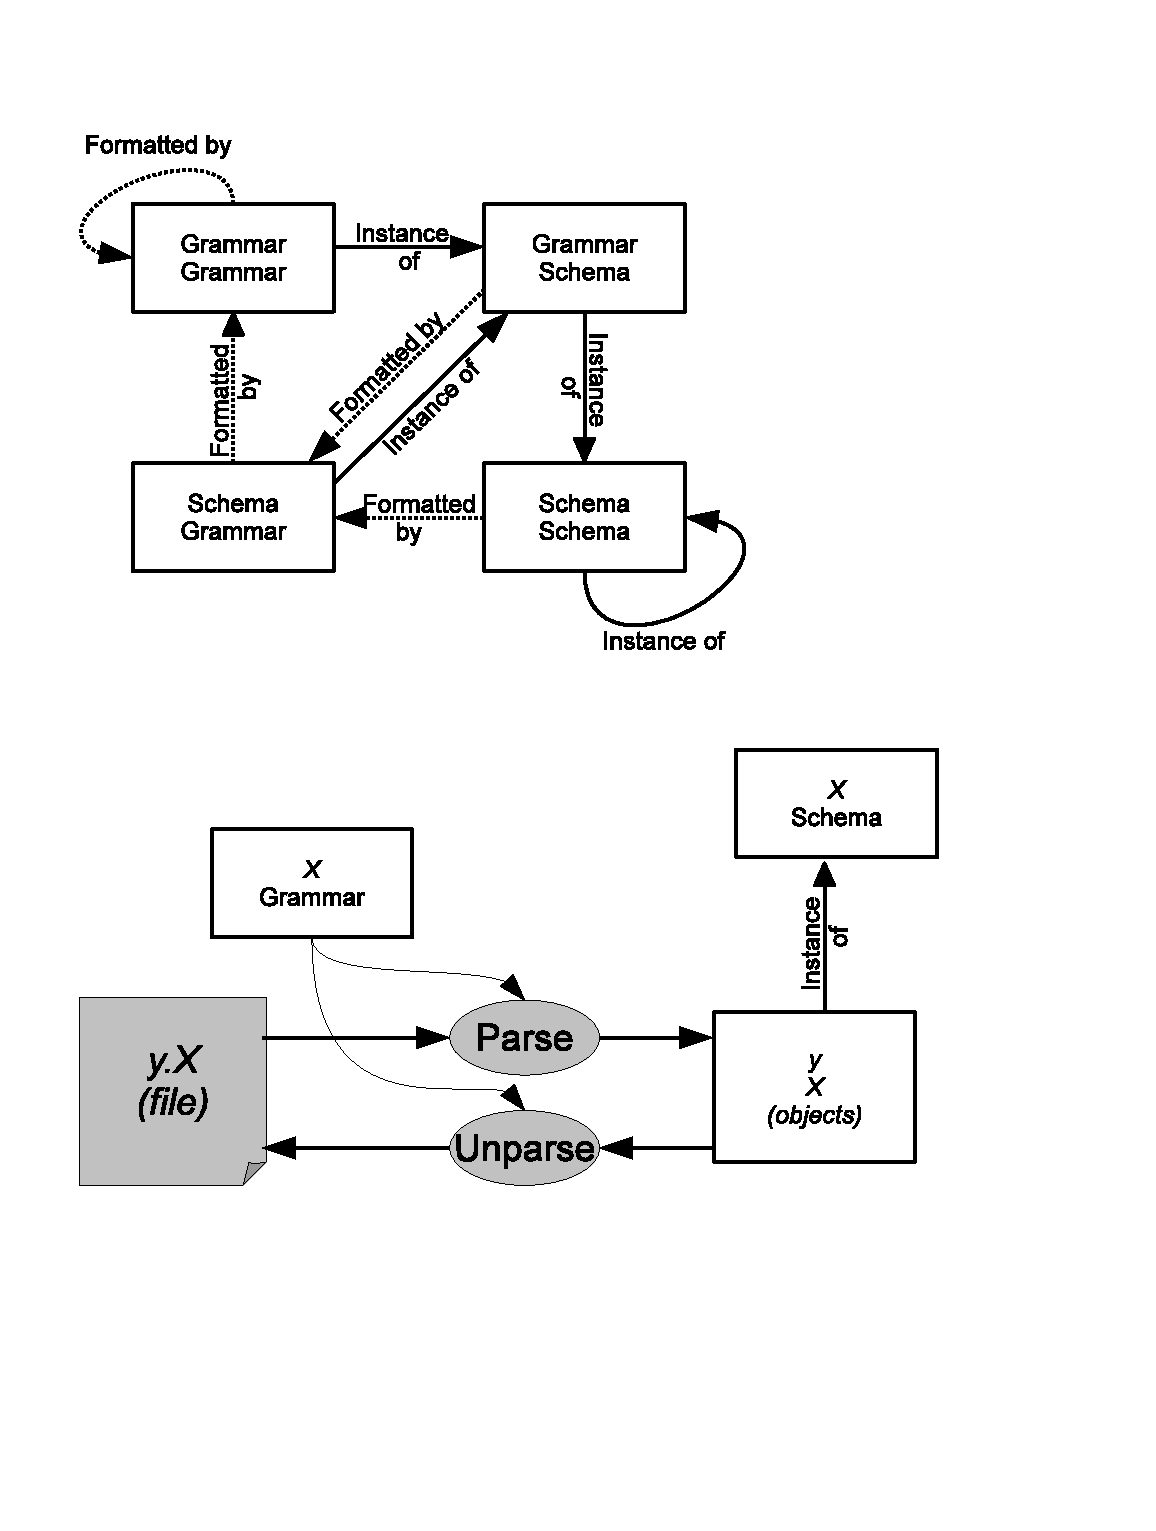
\includegraphics[scale=0.8]{QuadModel.pdf}
\caption{{\bf default}}
\label{default}
\end{center}
\end{figure}


\end{document}  



\begin{verbatim}
schema Geometry

class Shape

class Point < Shape
  x: int
  y: int

class Rectangle < Shape
  upper_left: Point
  lower_right: Point

class Circle < Shape
  center: Point
  radius: int

class Polygon < Shape
  points: Point*
  
class Composite < Shape
  items: Shape*
\end{verbatim}

It says that the class \C|Point| has fields \C|x| and \C|y|.
--------
This example converts schemas into constructor grammars
\begin{verbatim}
grammar NAME:sym
   CLASSES:
     rule NAME:sym = 
        (SUBTYPES: { NAME:sym "|") "|" @"!SUBTYPES.empty?")?
         [NAME:sym] NAME:str "{" 
            FIELDS: { (NAME:str ":" (NAME:sym): (
                 "[" { TYPE.NAME:sym^ "," } "]"   @"MANY=true"
               | TYPE.NAME:sym^ ?                  @"OPTIONAL=true"
               | TYPE.NAME:sym^
               )) ";" }
             "}"
\end{verbatim}
